\begin{frame}{Triangle Geometry}

\begin{minipage}[c]{0.85\textwidth}
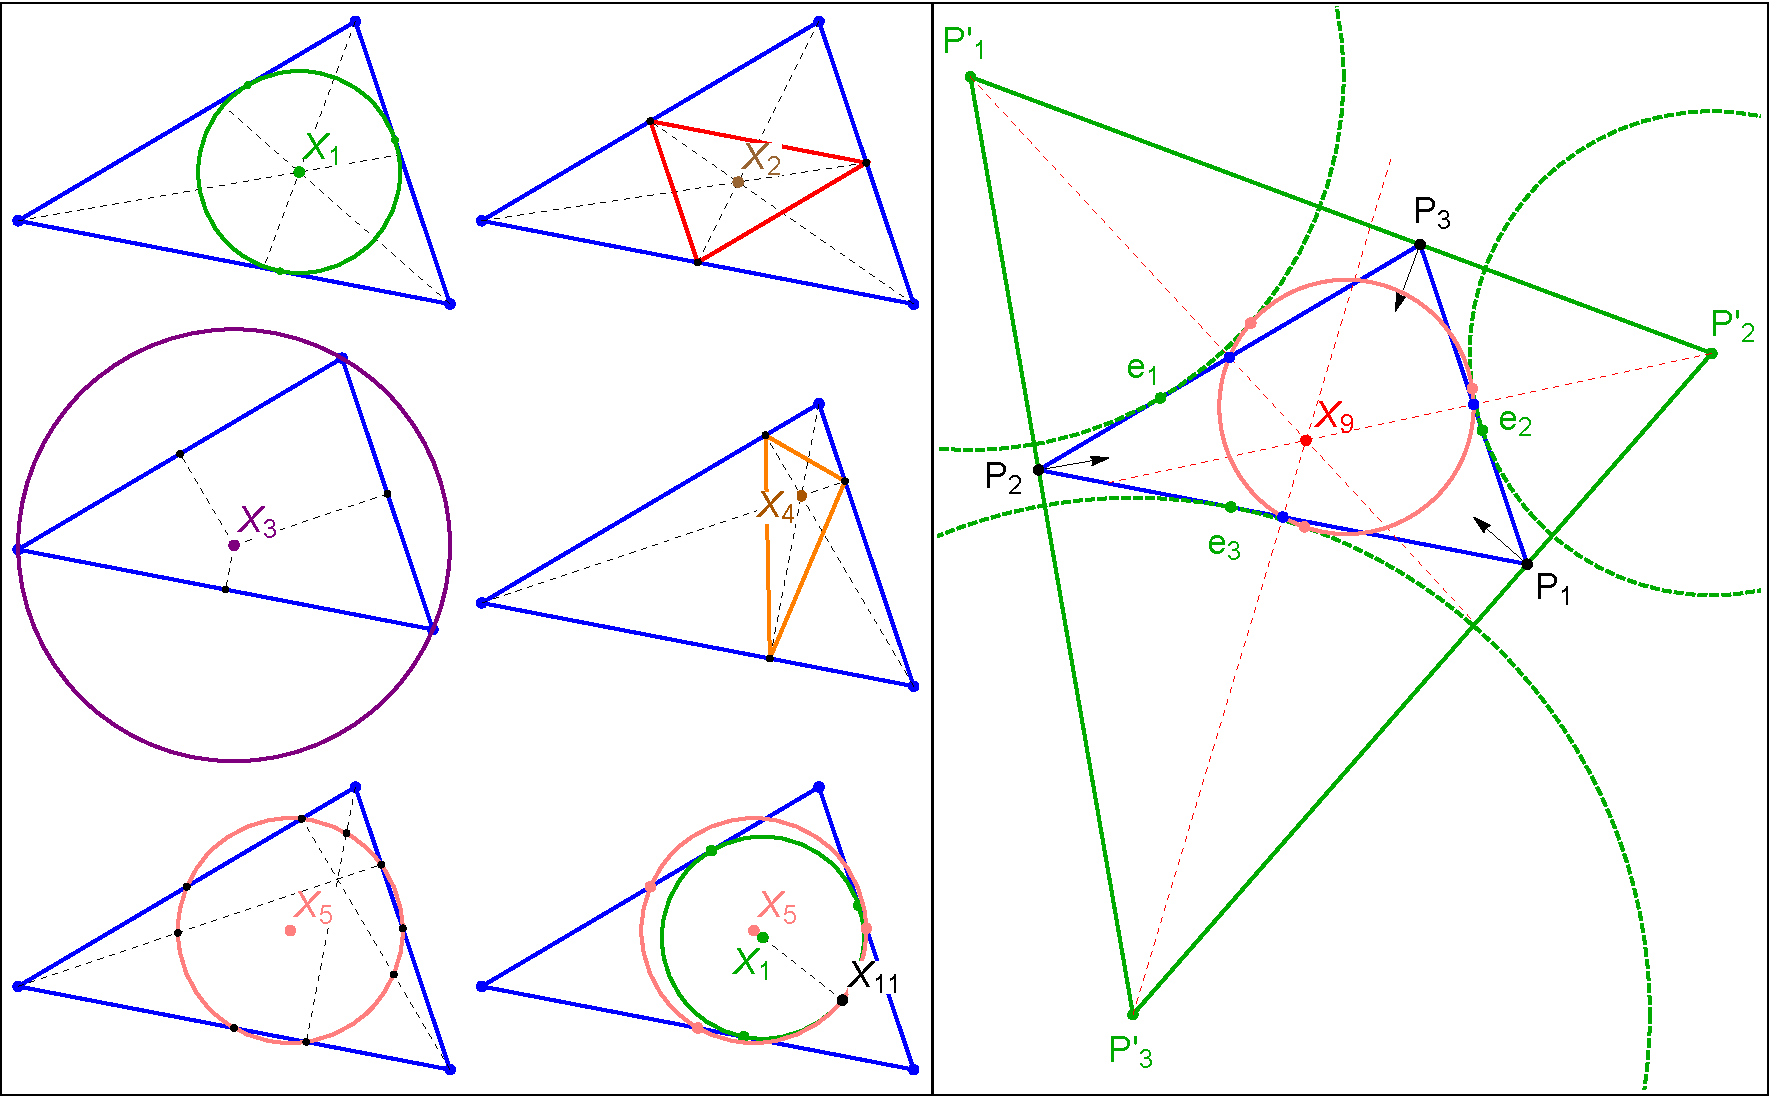
\includegraphics[width=.85\textwidth]{pics/0039_constr.pdf}
\end{minipage}
\hspace{-1.5cm}
\begin{minipage}[c]{.2\textwidth}
\begin{table}
\tiny
\begin{tabular}{p{1em}l}
$X_1$ & Incenter \\
$X_2$ & Barycenter \\
$X_3$ & Circumcenter \\
$X_4$ & Orthocenter \\
$X_5$ & 9-Point center \\
$X_9$ & Mittenpunkt \\
$X_{11}$ & Feuerbach Point
\end{tabular}
\end{table}
\end{minipage}
\end{frame}

\begin{frame}{Locus of Incenter is Elliptic \href{https://www.youtube.com/watch?v=BBsyM7RnswA}{[video]}}
\begin{figure}
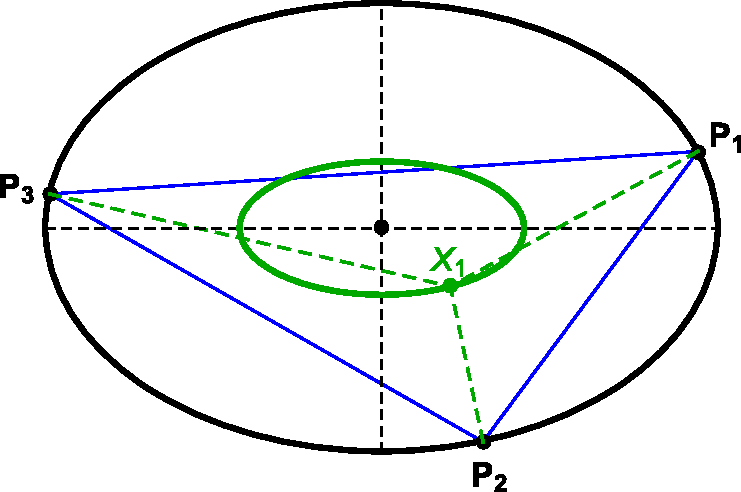
\includegraphics[height=.7\textheight]{pics/0020_incenter_locus.pdf}
\end{figure}
\end{frame}

\begin{frame}{Locus Intouch Points is Sextic \href{https://youtu.be/9xU6T7hQMzs}{[video]}}
\begin{figure}
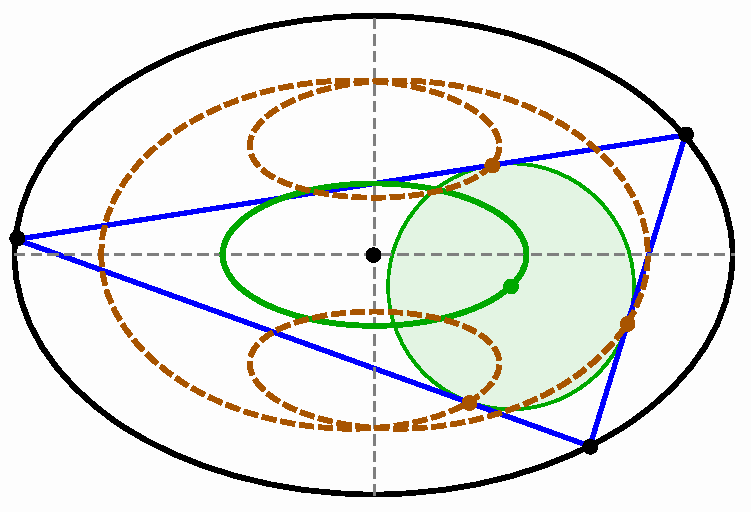
\includegraphics[height=.7\textheight]{pics/0001_intro_plot.pdf}
\end{figure}
\end{frame}

\begin{frame}{Interactive \href{https://editor.p5js.org/undefined/present/i1Lin7lt7}{Applet}}
\begin{figure}
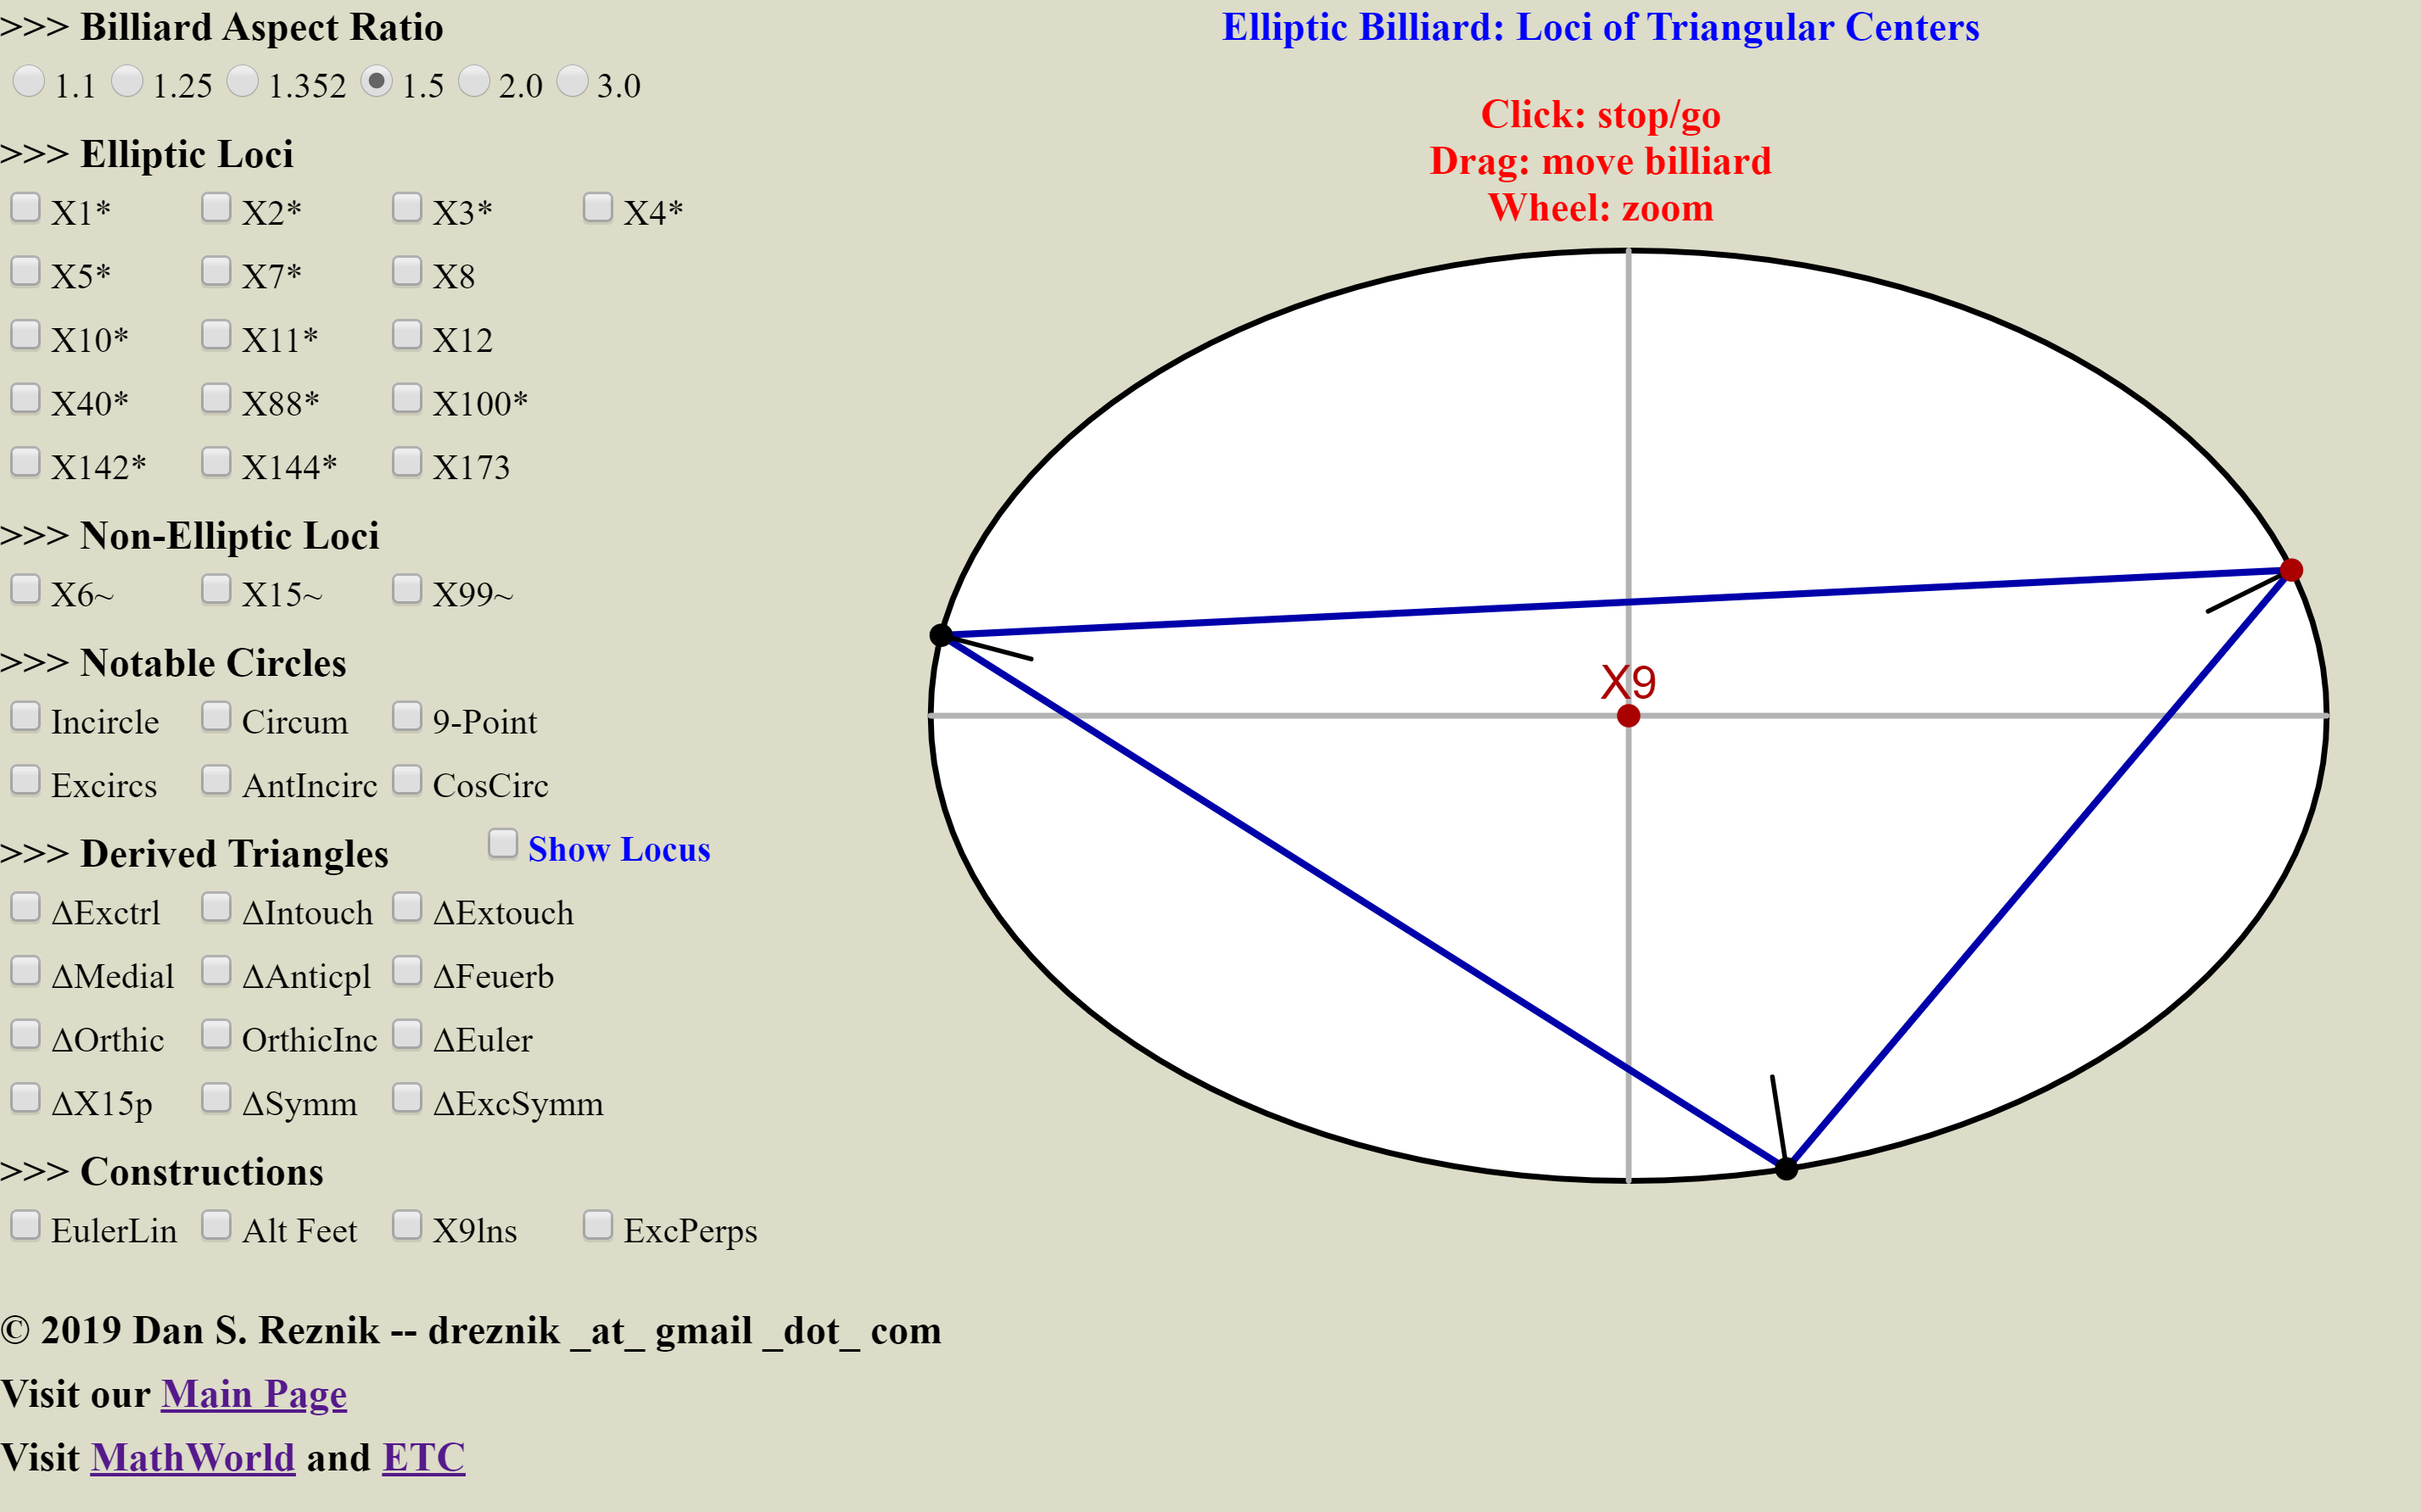
\includegraphics[height=.8\textheight]{pics/applet_p5js.png}
\end{figure}
\end{frame}  

\begin{frame}{Locus of Excenters is Elliptic \href{https://youtu.be/Xxr1DUo19_w}{[video]}}
\begin{figure}
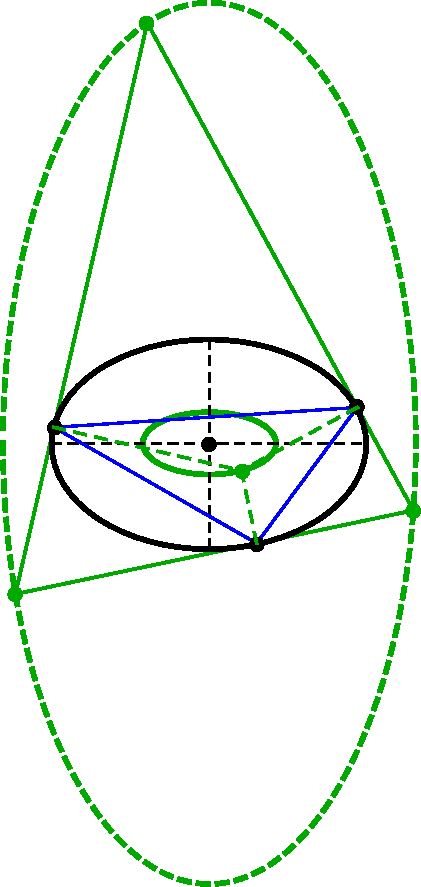
\includegraphics[clip,trim={0 4cm 0 0},height=.8\textheight]{pics/0025_incenter_excenter_locus.pdf}
\end{figure}
\end{frame}

%\begin{frame}{Major Triangular Centers}
%\begin{figure}
%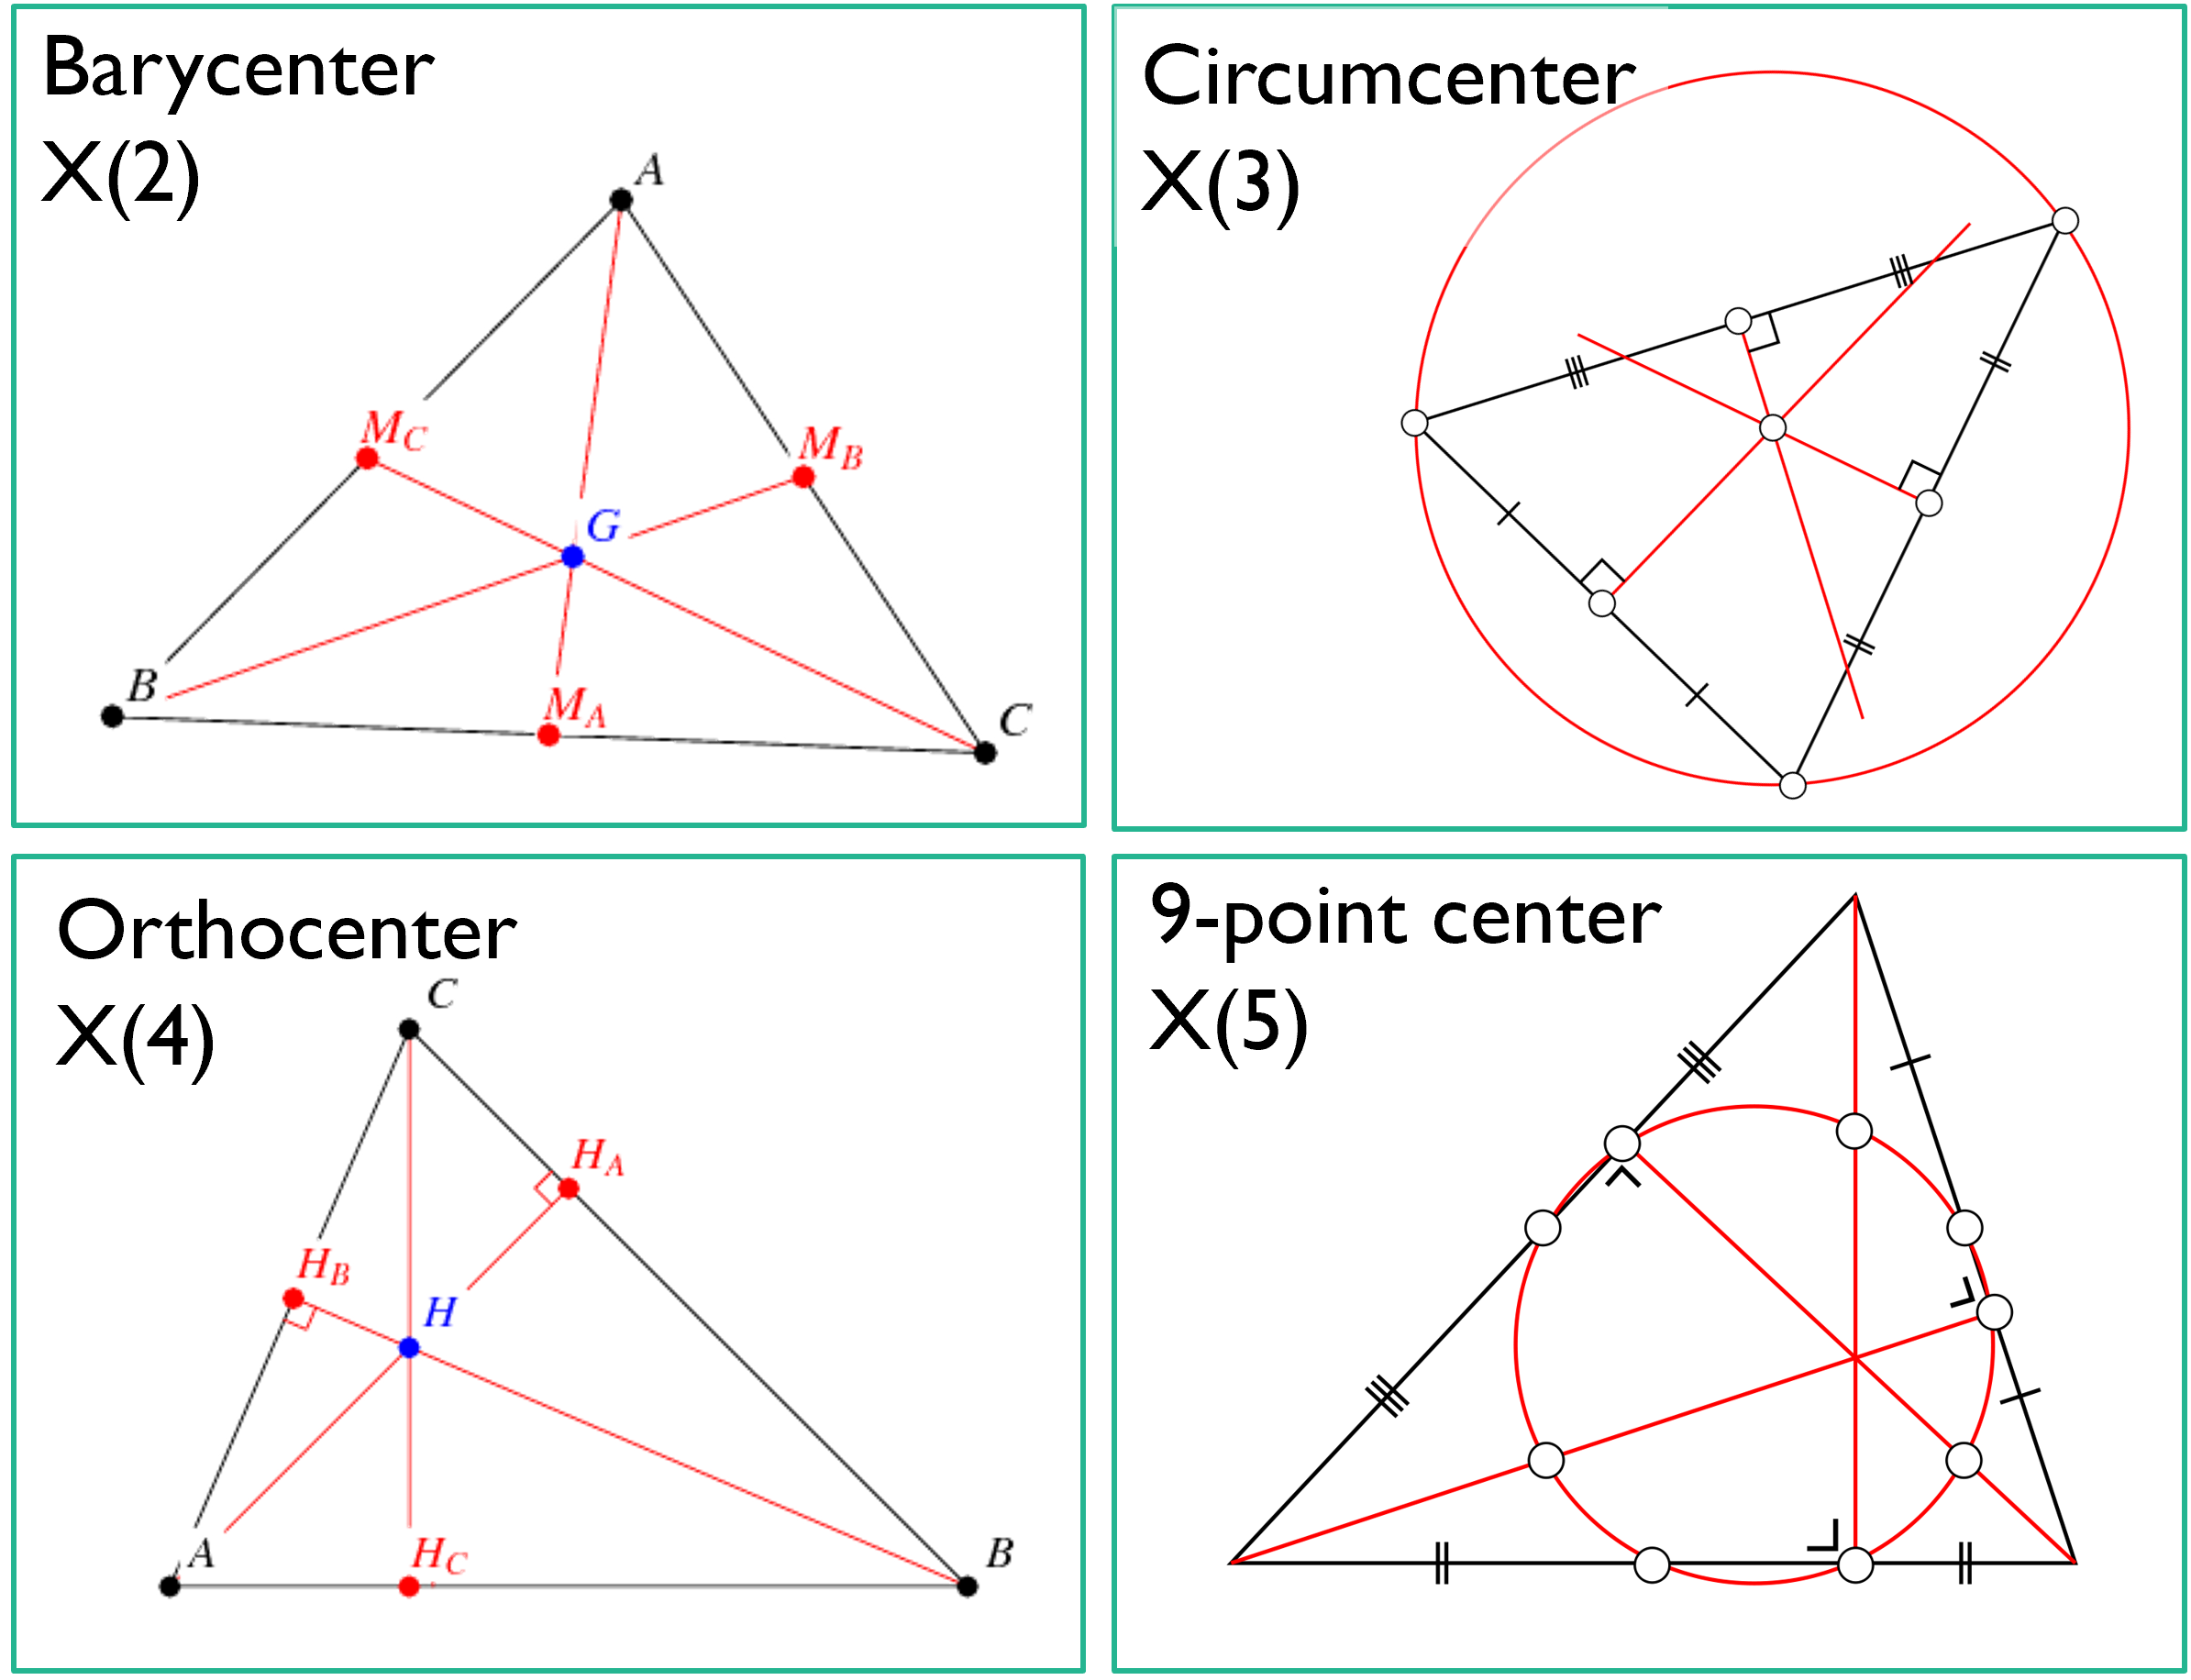
\includegraphics[height=.8\textheight]{pics/0000_major_centers.png}
%\end{figure}
%\end{frame}

\begin{frame}{Encyclopedia of Triangular Centers \href{https://faculty.evansville.edu/ck6/encyclopedia/ETC.html}{[ETC]}}
\begin{figure}
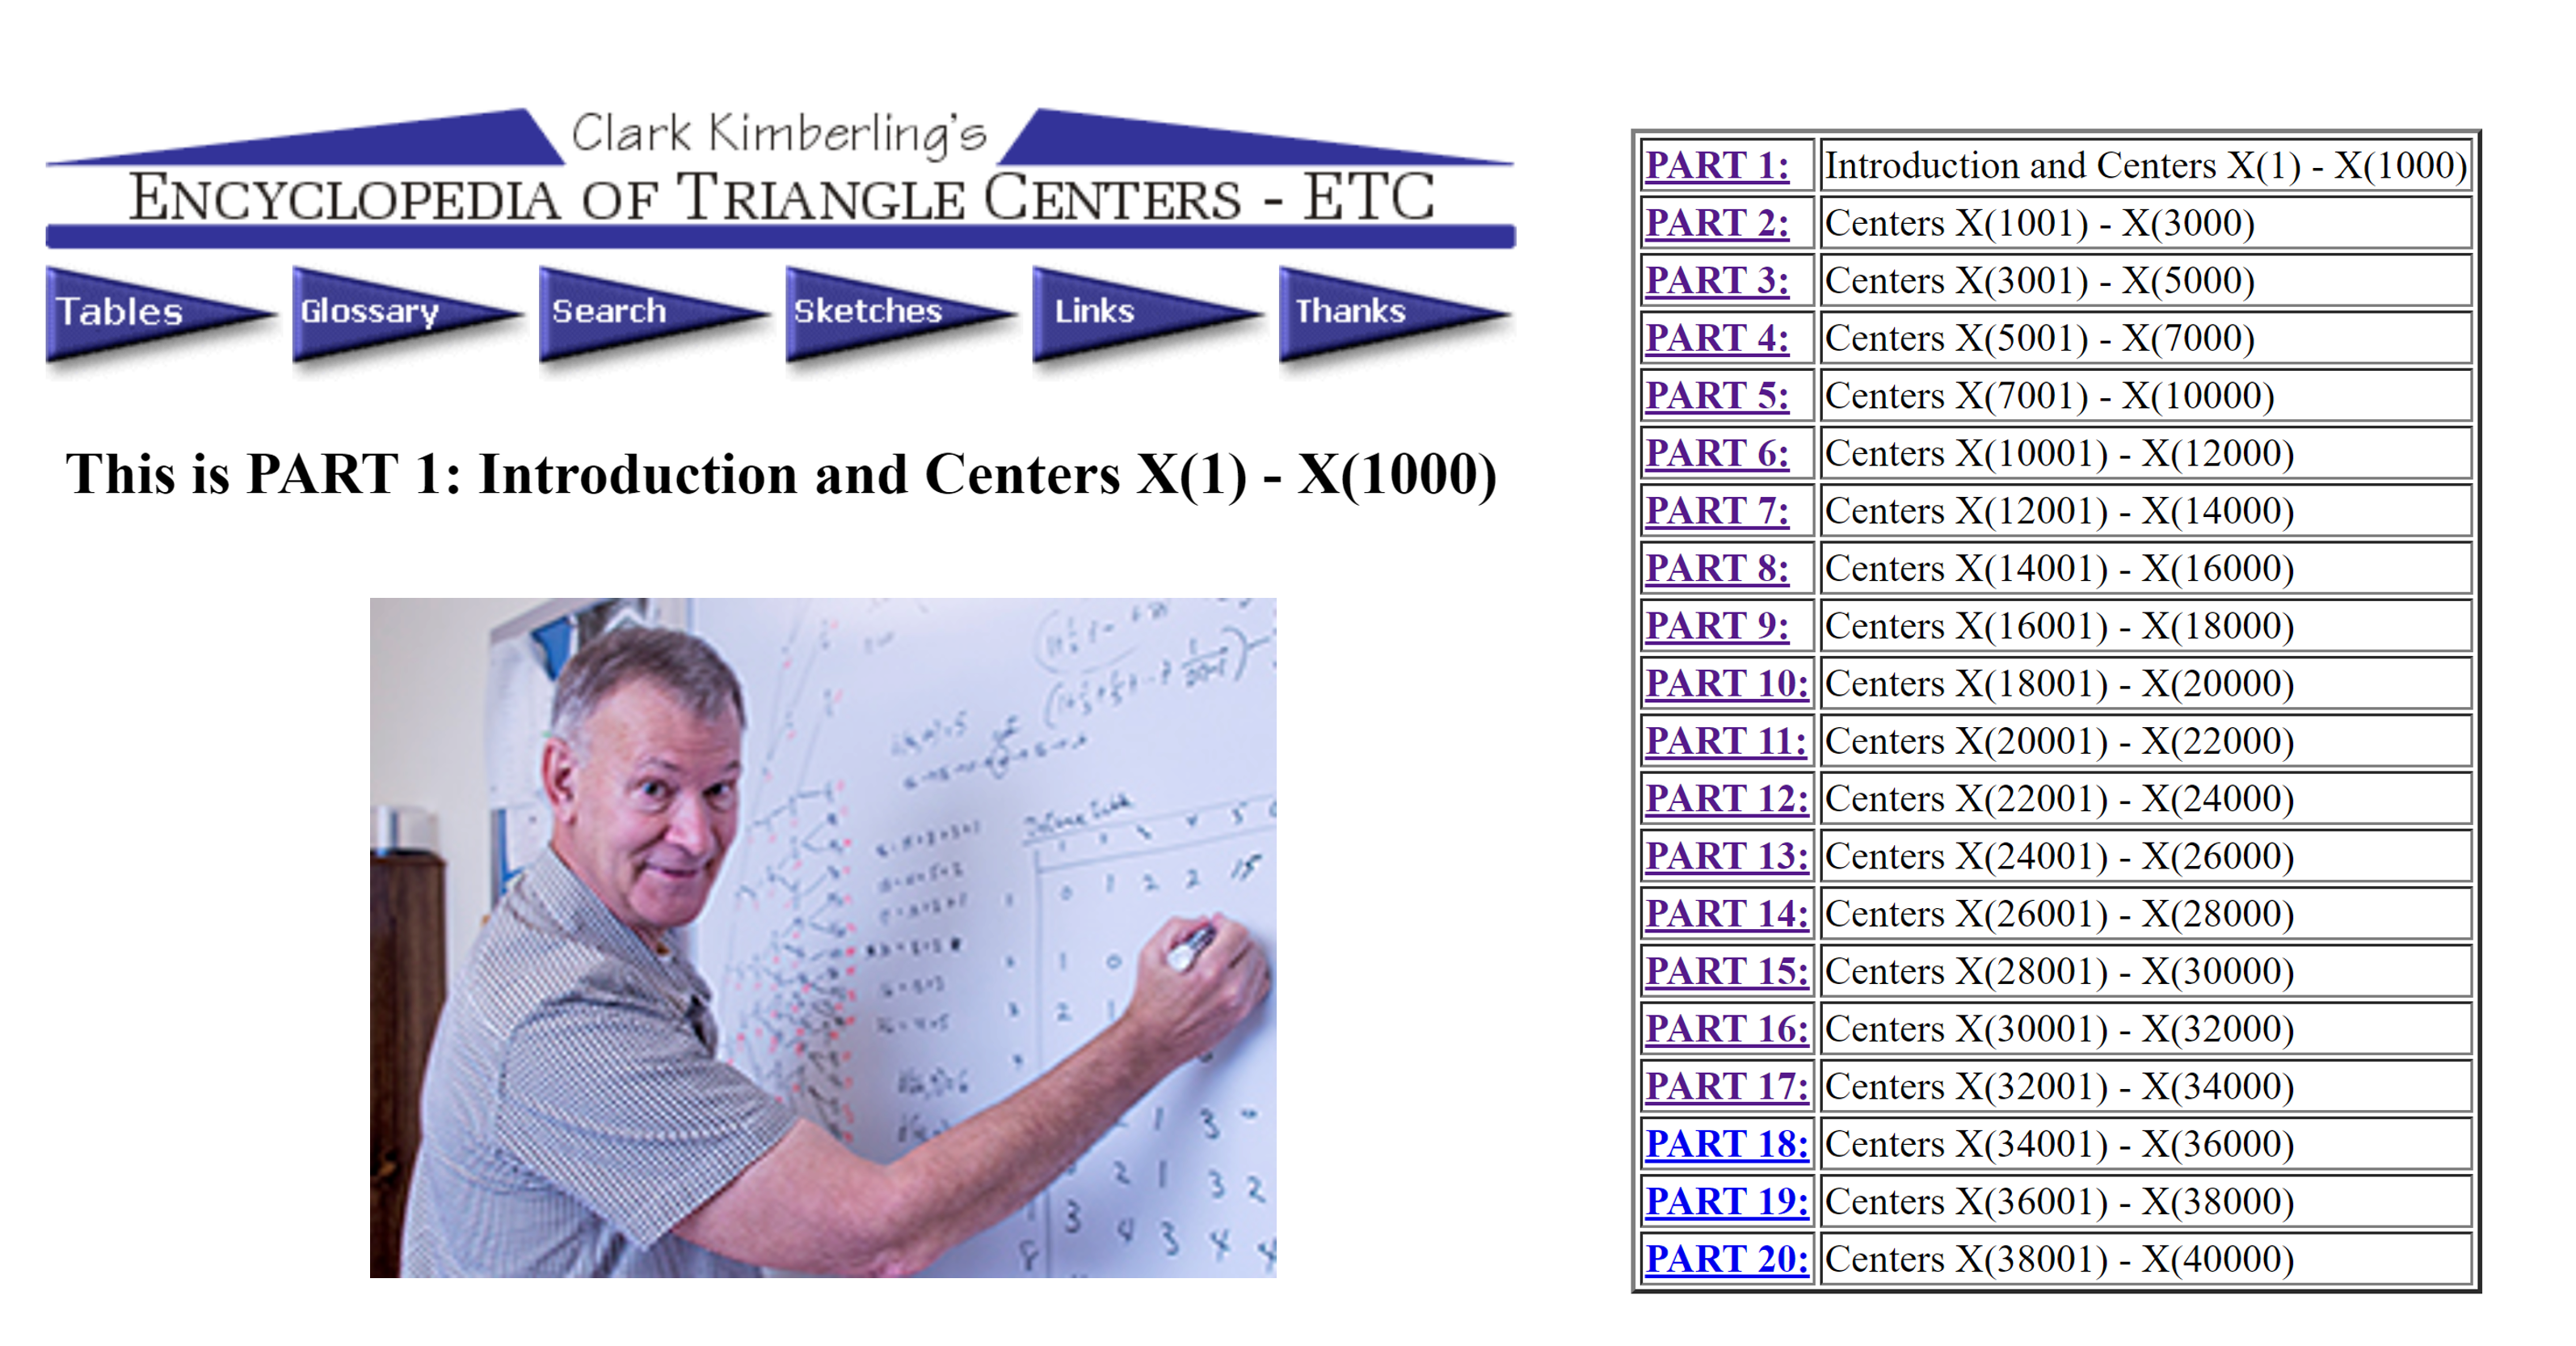
\includegraphics[height=.8\textheight]{pics/0000_etc.png}
\end{figure}
\end{frame}

\begin{frame}{Elliptic Loci of Major Triangular Centers \href{https://youtu.be/sMcNzcYaqtg}{[video]}}
\begin{figure}
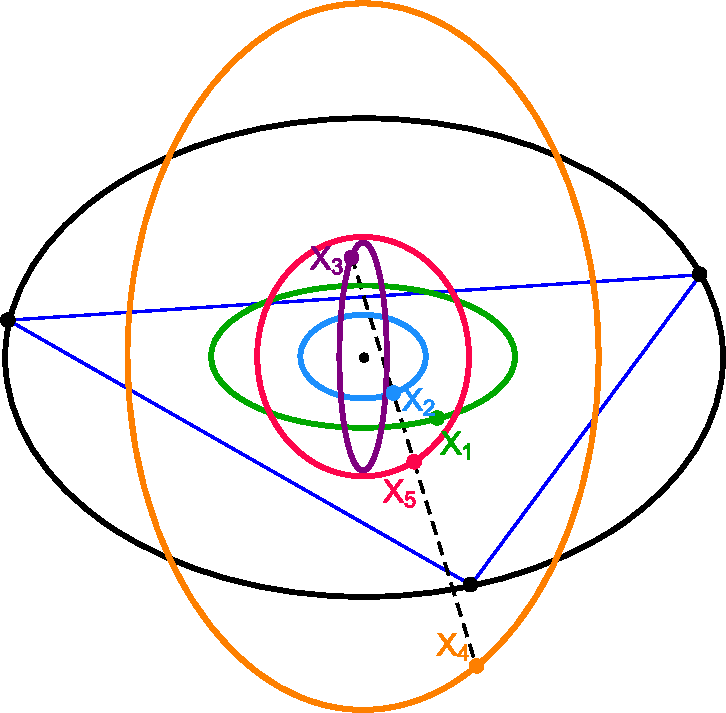
\includegraphics[height=.75\textheight]{pics/0030_x12345_locus.pdf}
\end{figure}
\end{frame}

\begin{frame}{Derived Triangles \href{https://youtu.be/xyroRTEVNDc}{[video]}}
\begin{figure}
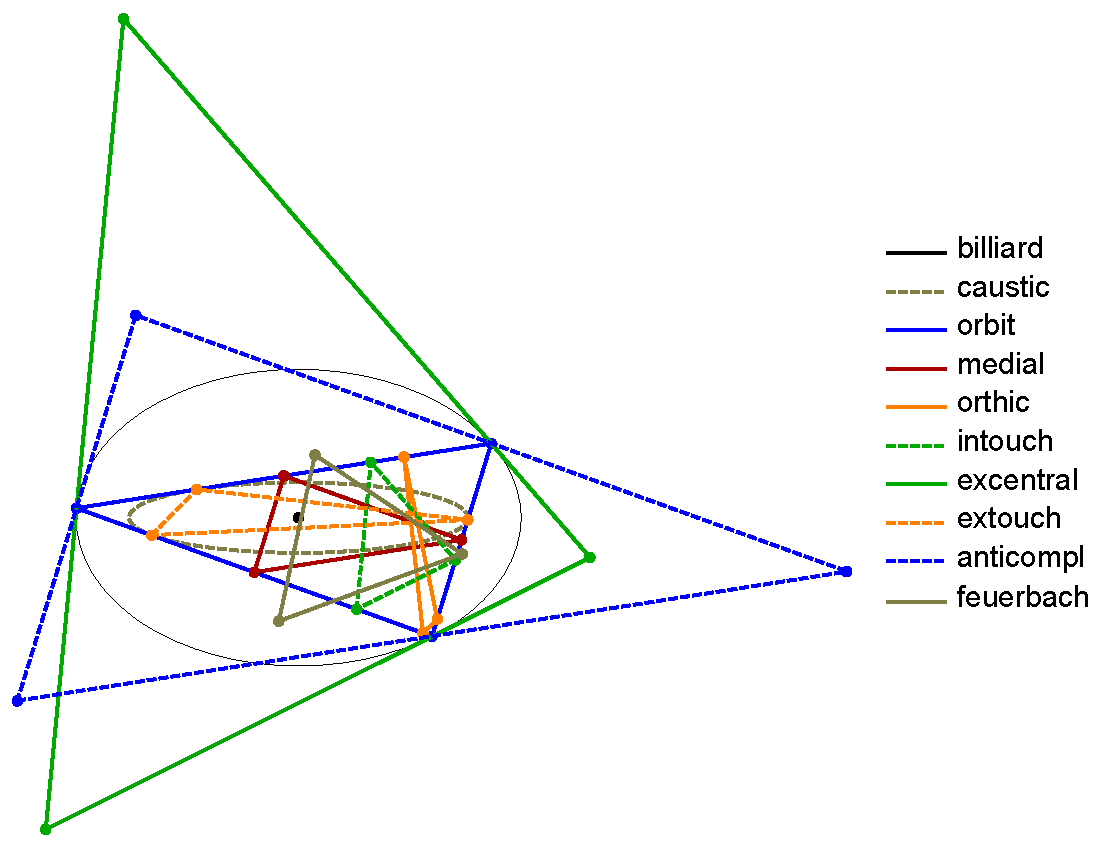
\includegraphics[clip,trim={0 0 0 3cm},height=.8\textheight]{pics/0043_derived-triangles.pdf}
\end{figure}
\end{frame}

\begin{frame}{Loci of Vertices of Derived Triangles \href{https://youtu.be/OGvCQbYqJyI}{[video]}}
\begin{figure}
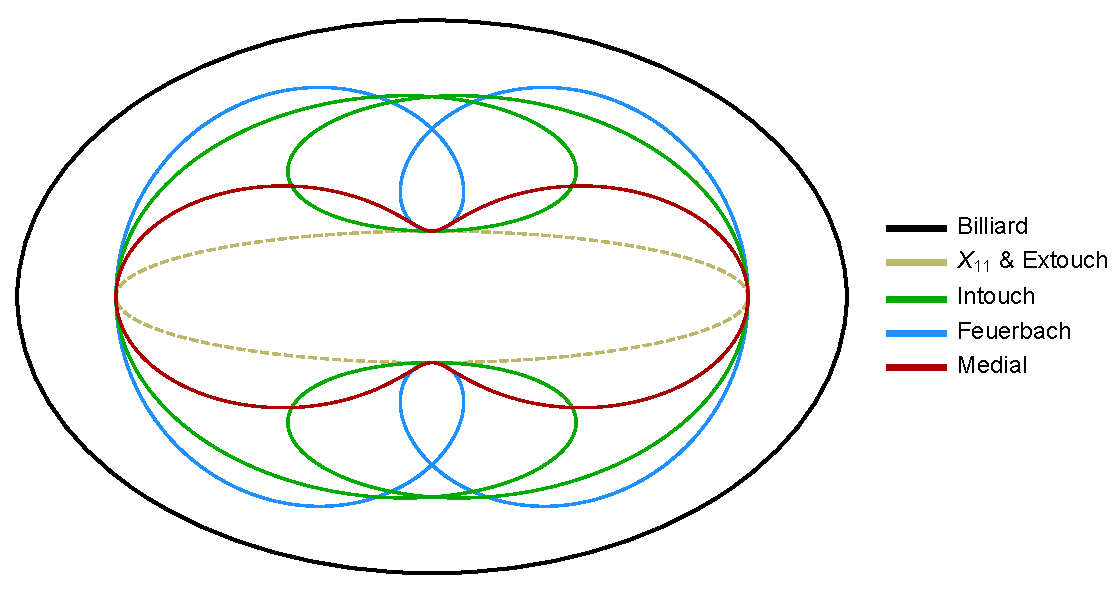
\includegraphics[height=.7\textheight]{pics/0040_non_elliptic.pdf}
\end{figure}
\end{frame}

\begin{frame}{Feuerbach, Anticomplement, and Extouchpoints \href{https://youtu.be/TXdg7tUl8lc}{[video]}}
\begin{figure}
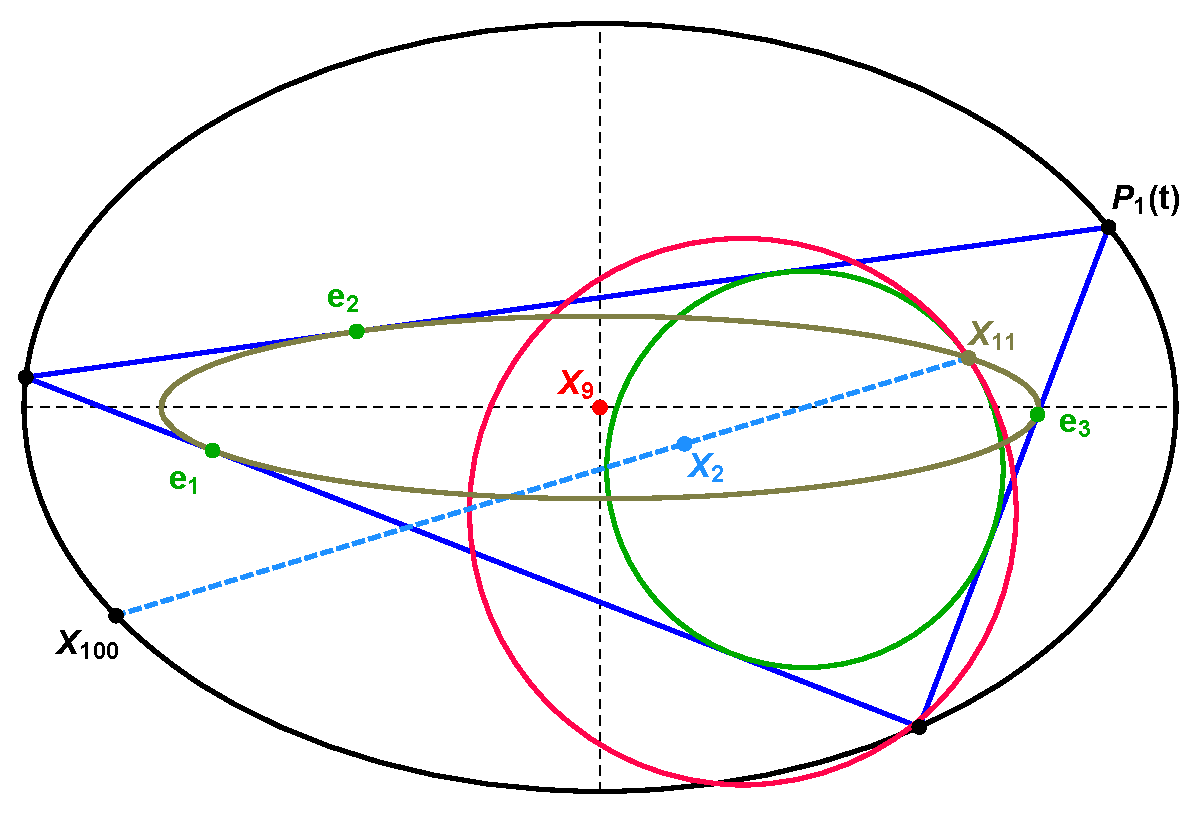
\includegraphics[height=.75\textheight]{pics/0035_feuerbach_loci.pdf}
\end{figure}
\end{frame}

\begin{frame}{Symmedian Point: Quasi-Elliptic Convex Quartic}
\begin{tabular}{rl}    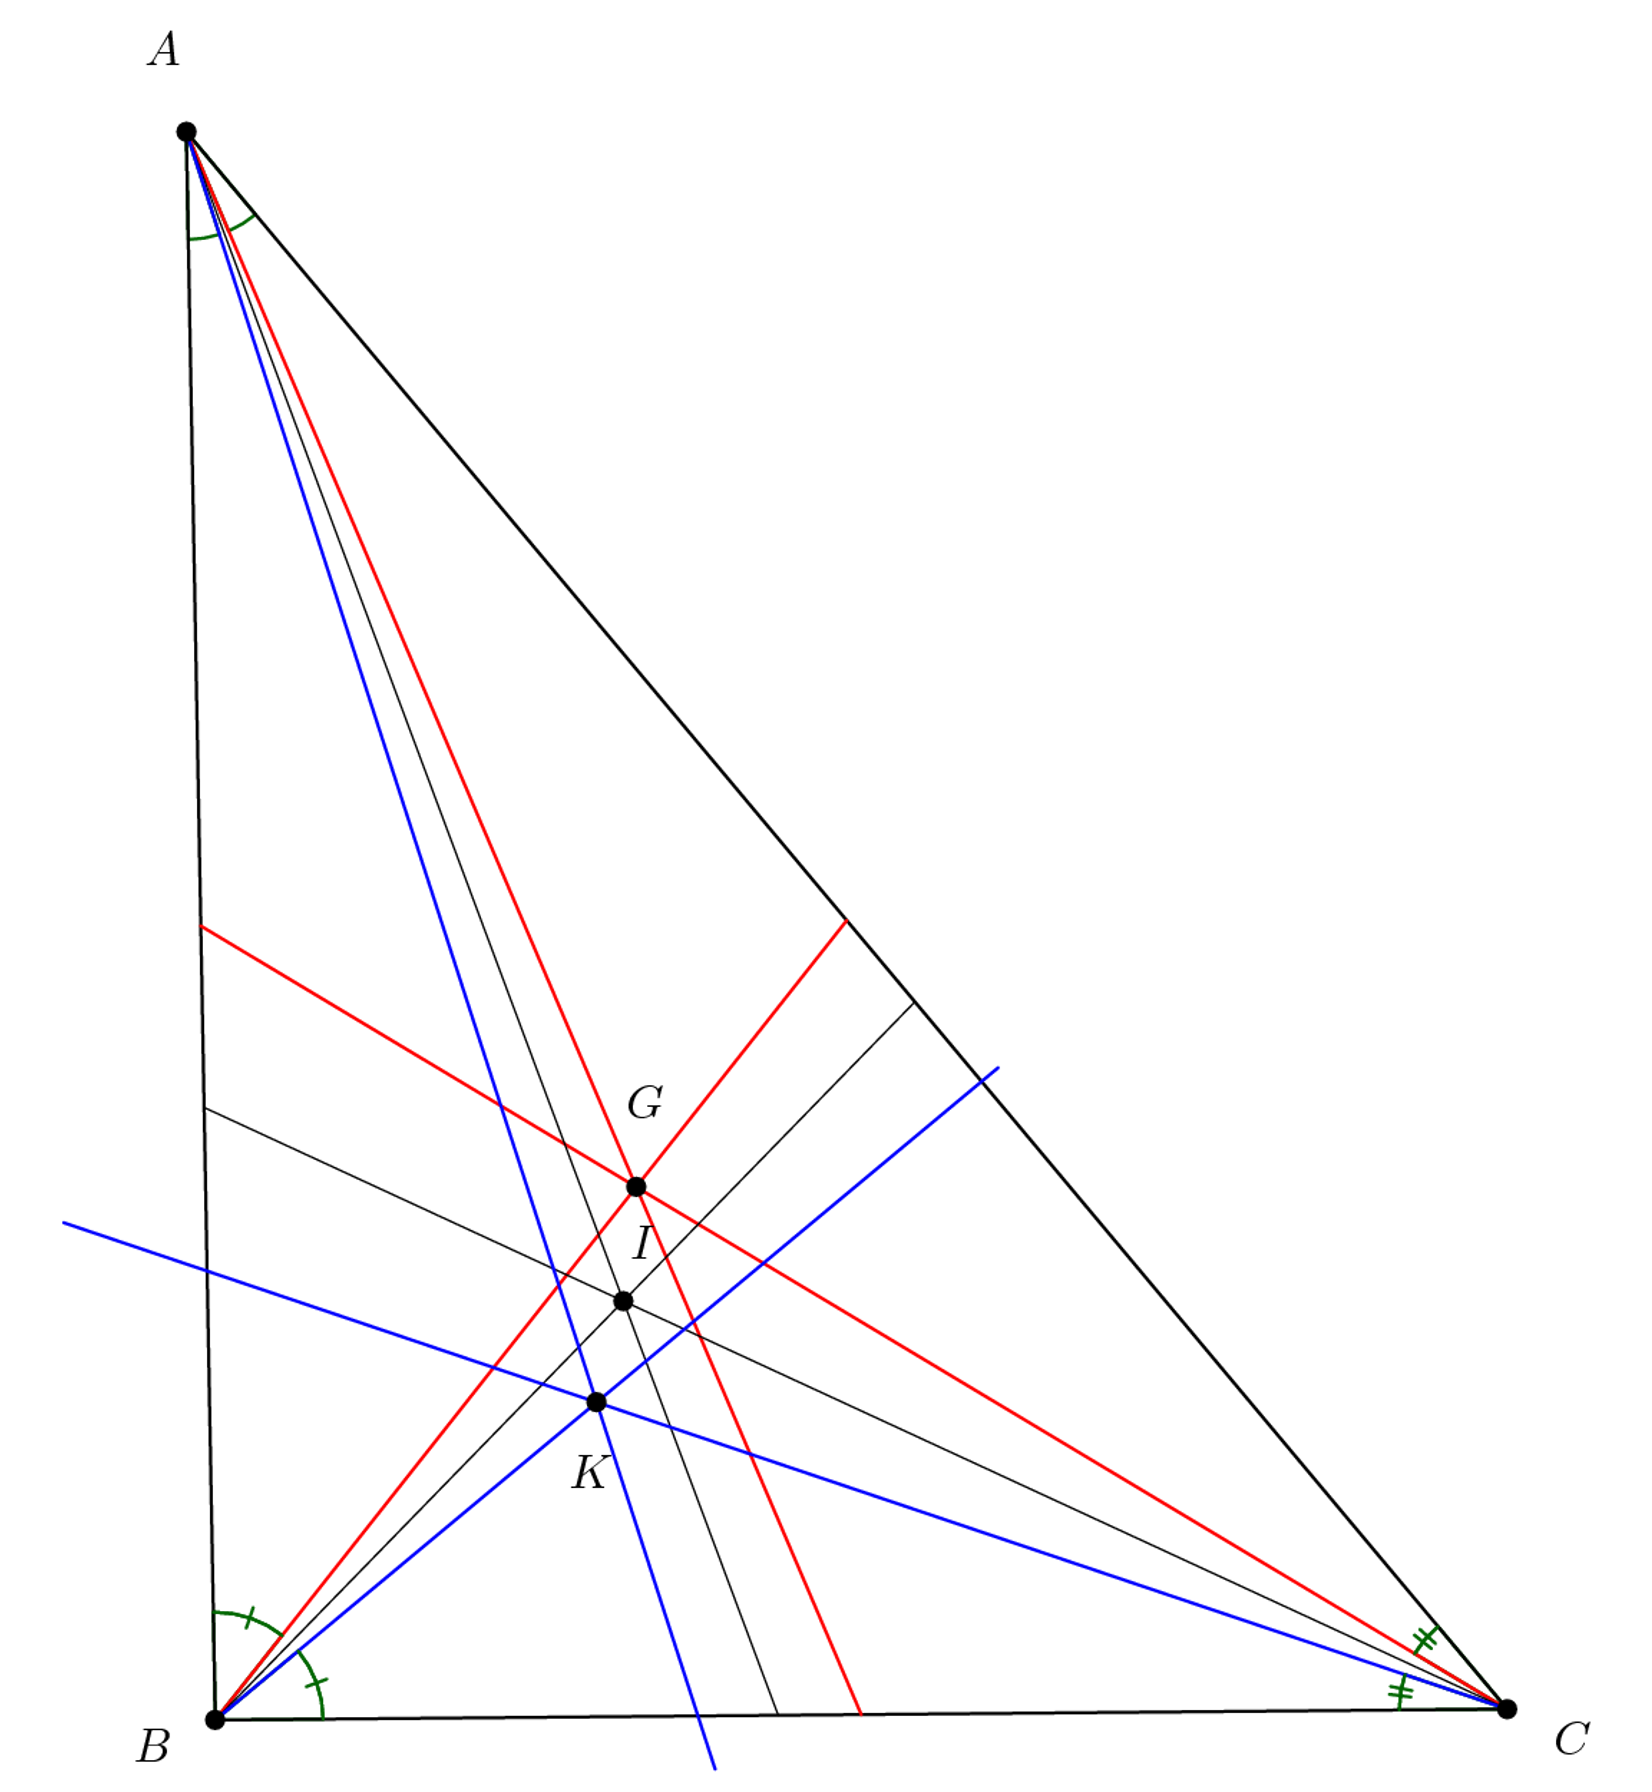
\includegraphics[width=.4\textwidth]{pics/0000_symmedian.png} & \hspace{-1cm} 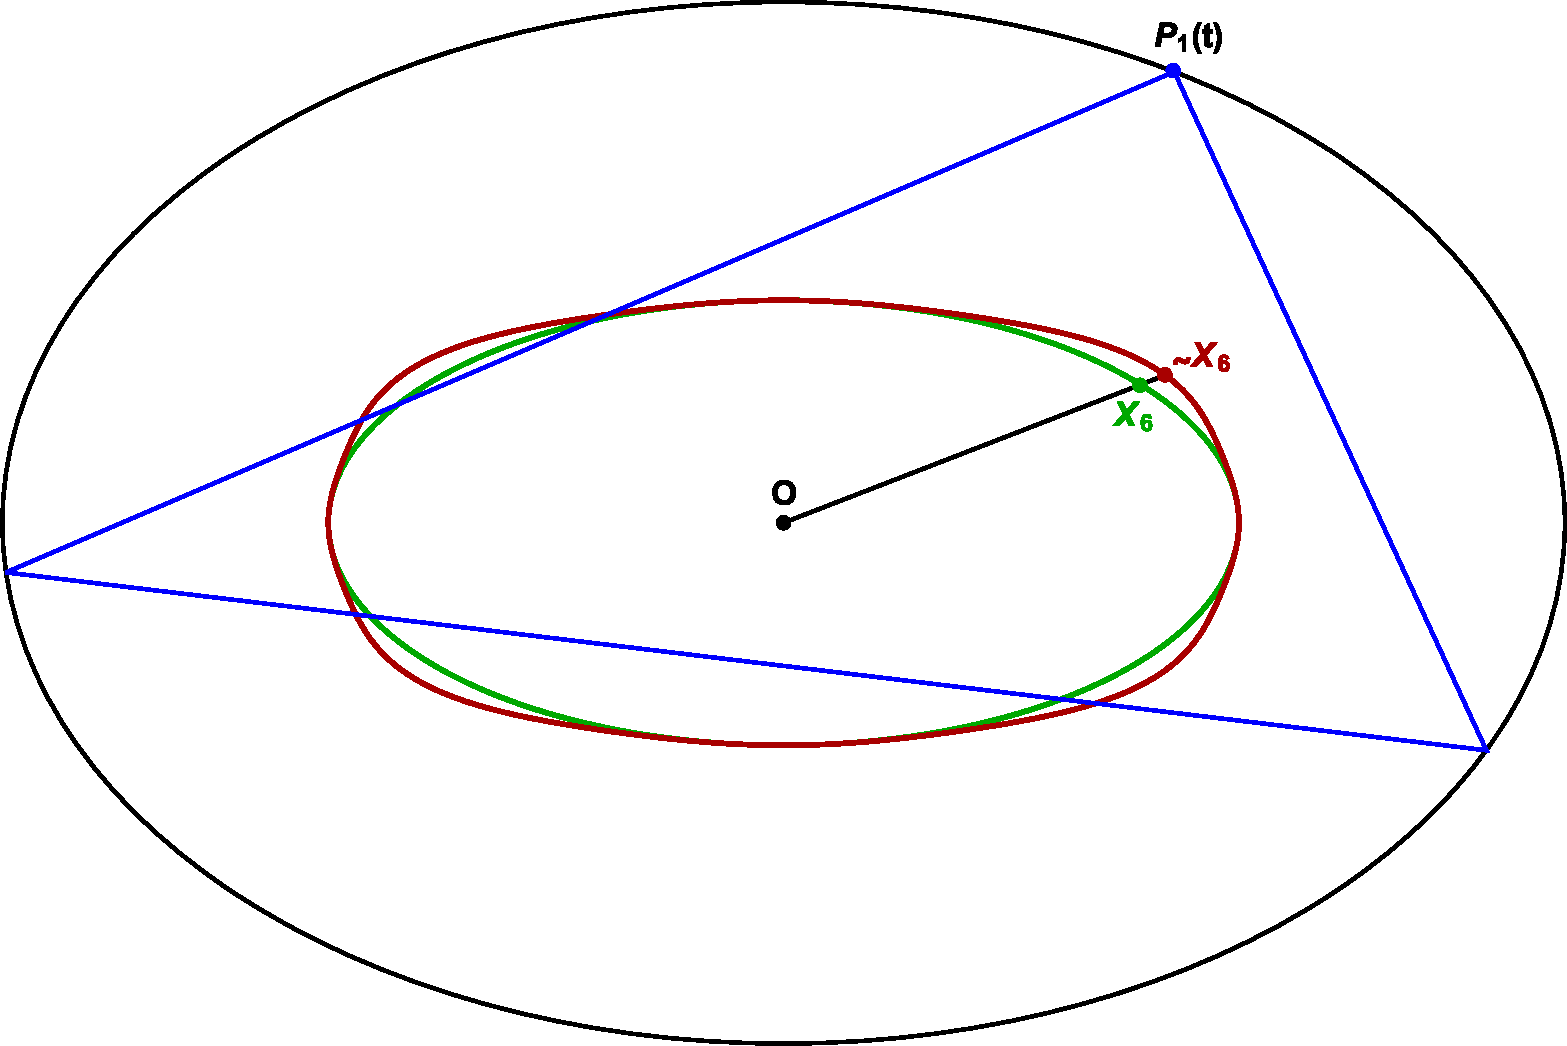
\includegraphics[width=.6\textwidth]{pics/0041_symmedian.pdf}
\end{tabular}
\end{frame}

\begin{frame}{Orthic Incenter: Four Kinks \href{https://youtu.be/3qJnwpFkUFQ}{[video]}}
\begin{figure}
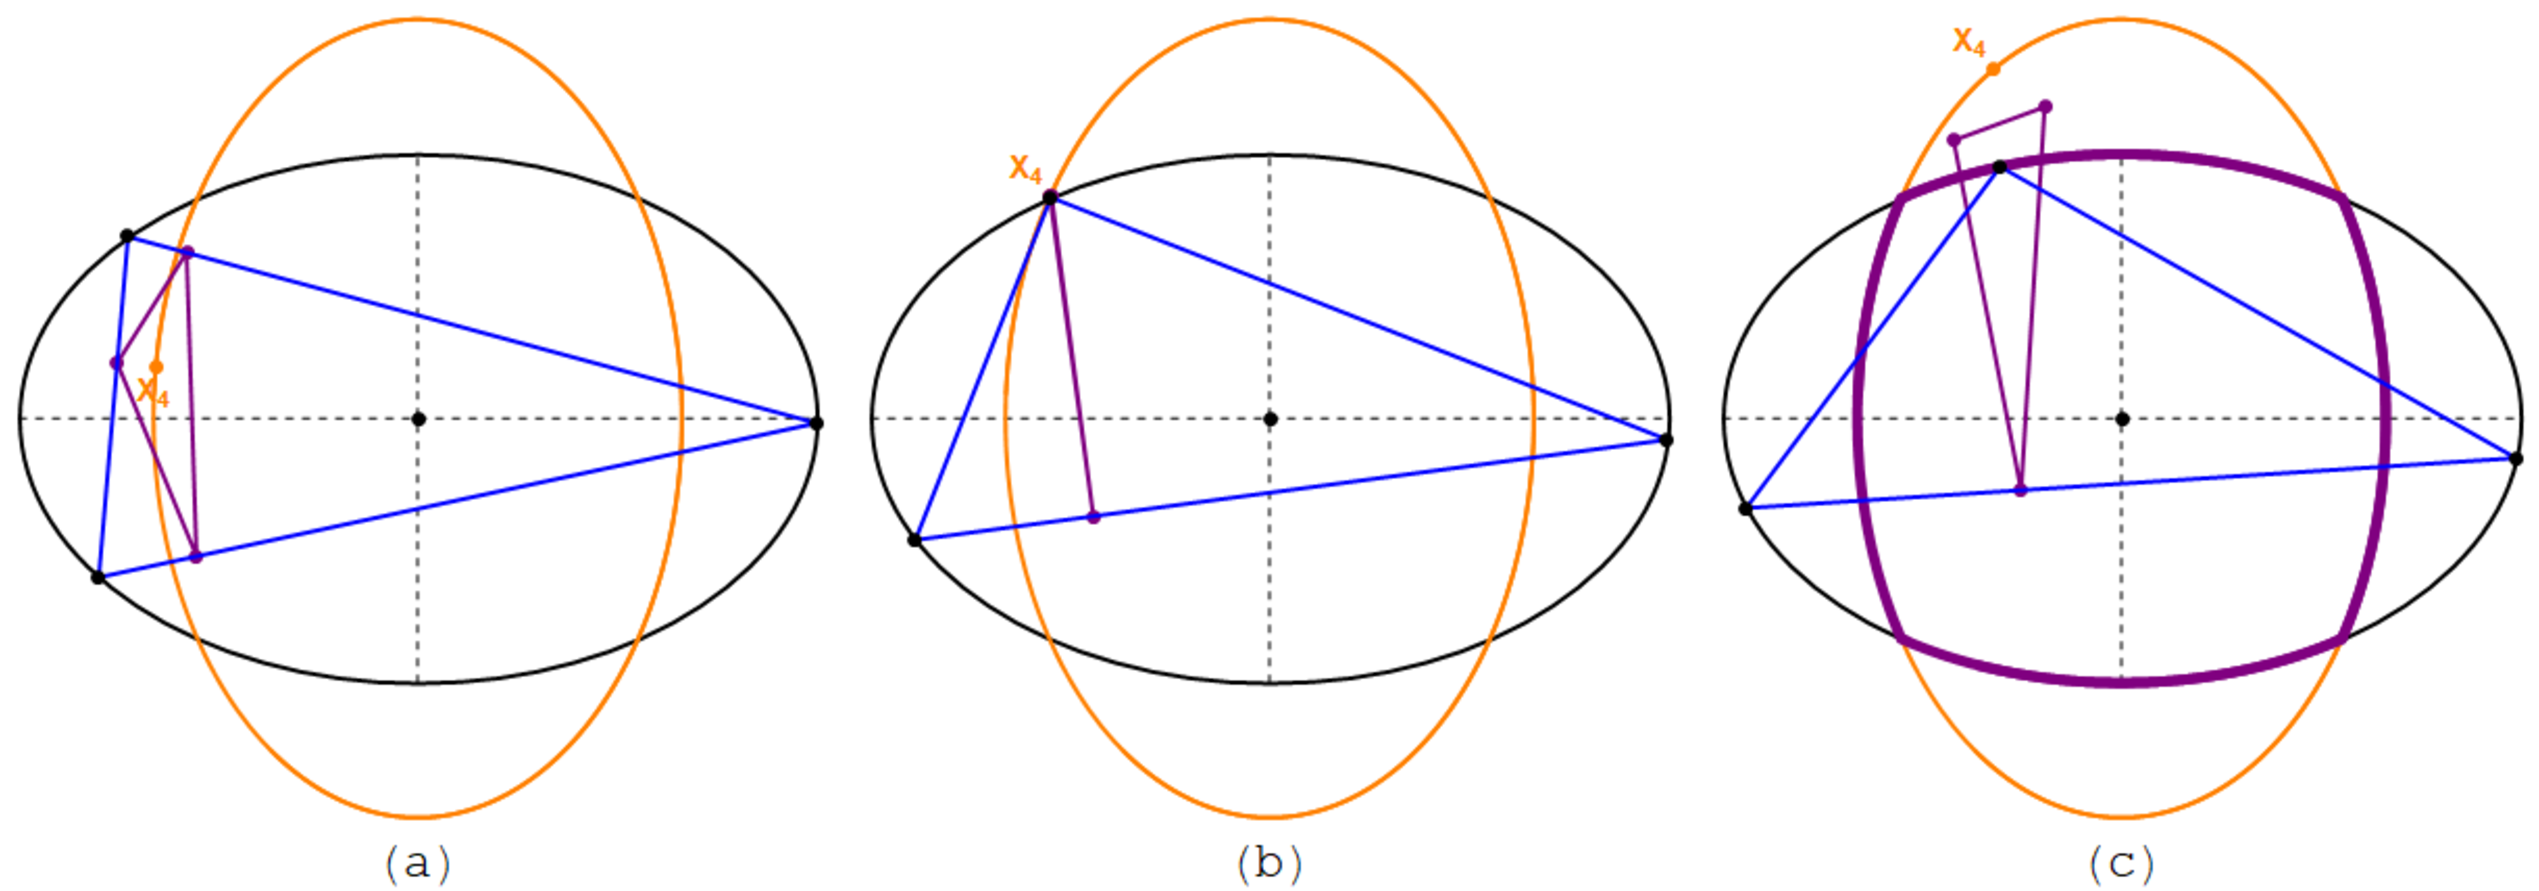
\includegraphics[width=\textwidth]{pics/0045_ort_loci_orthic.pdf}
\end{figure}
\end{frame}

\begin{frame}{Intouchpoints of Anticomplementary Track Billiard \href{https://youtu.be/50dyxWJhfN4}{[video]}}
\begin{figure}
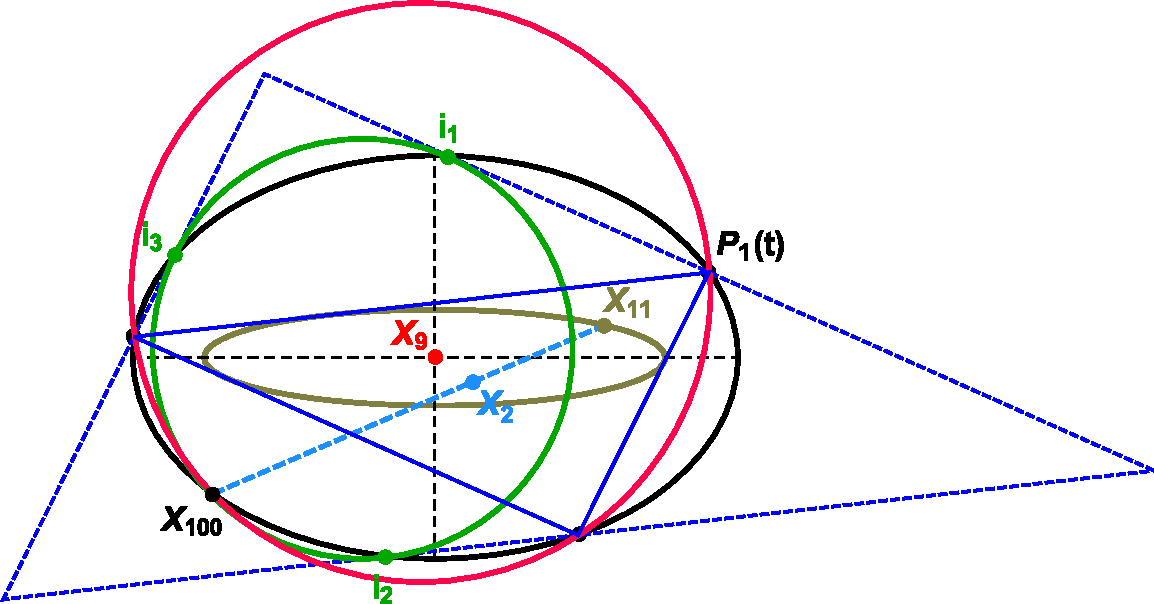
\includegraphics[height=.7\textheight]{pics/0048_act_intouch.pdf}
\end{figure}
\end{frame}

\begin{frame}{A Circular Locus! \href{https://youtu.be/hCQIT6_XhaQ}{[video]}}
\begin{tabular}{rl}
\begin{tabular}{r}
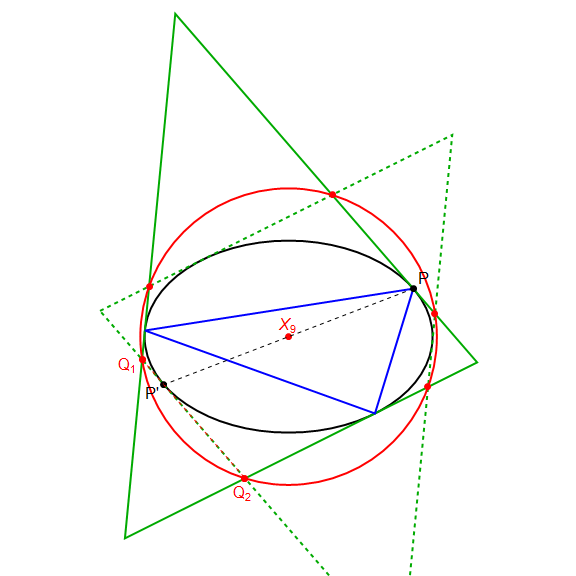
\includegraphics[height=.8\textheight]{pics/0120_cosine_circle_reflected_excentral.png}
\end{tabular} & \hspace{-1cm}\begin{tabular}{l}
\parbox{0.5\linewidth}{
  \begin{minipage}{0.45\textwidth}
  $$r^* = \frac{1}{\gamma}$$ \end{minipage}}
\end{tabular}  \\
\end{tabular}
\end{frame}